\section{Motivating Prices}

While \(\bar{X}_n\) is great to build intuition about societies of people, all
its elements are \(n\)-th portions of some total production vector \(x\in X\).
This suggests that everyone would consume the exact same things. And while
clones are great and all, that is not what we are interested in. So how could
multiple people share the goods they produced, without necessarily consuming the
exact same things? 

To satisfy the ``Pluralism in Economics'' crowd, let us avoid
the term ownership for now. We simply observe that some people will produce
things and not necessarily the same people will consume\footnote{
	You can turn a product you can use \(m\) times (before it breaks down)
	without loss of generality into a consumable, by considering these \(m\) uses
	to be individual products. So a person does not ``have'' a chair, but rather
	the \(i\)-th usage of said chair. With this trick in mind, all products are
	consumable.
} the products.
No matter how you organize a society, from an individual perspective, there
are going to be goods the individual \(i\) produces \(S_i\in\real^\dims\) and
goods the individual consumes \(D_i\in\real^\dims\). And fundamentally a
society cannot consume more than is produced (and probably does not want to
produce more than necessary), so we need
\[
	S = \sum_{i=1}^n S_i = \sum_{i=1}^n D_i = D.
\]
The big question is: how can we ensure this? We also want everyone to
voluntarily participate in society. And people are going to stop doing so, if
they feel ripped off as they contribute much more than they get back.
Unfortunately it is difficult to compare the size of two vectors \(S_i\) and
\(D_i\) of uncomparable products. Of course we could enforce \(S_i=D_i\), but
then we are back to hermits, since everyone is using only what they produce.

To make the products comparable again, we could measure them by the time it took
to produce them. In other words the effort required for them. But recall that
the time needed to produce good \(j\), \(l_i^{(j)}\), might be different for
every person \(i\). Additionally this time is private information of person
\(i\). Especially if we generalize it to be a discomfort measure instead of
strictly time.


\begin{example}[Definitely not Capitalism]
	\label{ex: Definitely not Capitalism}
	Let us try to build a communist utopia, without money and ownership.  For
	this assume that the person which produces good \(j\) jots down their
	subjective cost of production \(l_i^{(j)}\) and tags the product with it and
	puts it into a communal holding space. Additionally they add the cost to
	their ``work-time'' tally.  Whenever someone wants to consume the product,
	they add the cost to their ``consumption-time'' tally, and take the product
	from communal holding space.  Everyone makes sure that their ``work-time''
	tally is comparable to their ``consumption-time''. We have tags, because
	people are bad at estimating how much effort is behind the products they
	consume.

	Does this sound like a utopia? Great!
	We can simplify the two tallies into one, because we only want to make
	sure that the difference is approximately zero. So we might as well add
	``work-time'' and subtract ``consumption-time'' from the get go. We also do not
	need to know how the current tally came to be, so we only need to keep track
	of the running total. This total is going to fluctuate around zero. When it
	is positive, you have worked more for society than you have consumed. And
	vice versa when it is negative.

	Now consider the life of a single product. When it is consumed, the cost was
	added to the tally of the producer and subtracted from the consumer. If you
	had chips to represent the tally, then they would have been simply passed from
	the consumer to the producer. Oh, wait! That's money! People are trading goods
	for money!

	Although right now, tallies can be negative and we do not have negative
	chips/money. This is a problem if you start out with everyone at zero. Because
	nobody can go below that. Or can they? If Alice signs a piece of paper saying
	she owes \(x\) amount of work-time, then she can pass that for a product that
	costs \(x\). The person receiving this note could then pass this note on to
	pay for something too. And if everyone trusts Alice, this is going to go
	swimmingly. So in principle anyone can create money. Money is just the debt
	of someone. The difficulty is creating debt which is widely accepted.

	The balance on a bill splitting app is money (in your friends circle), a coupon
	is money (scammers like to be paid in it), etc. But the money which is most
	widely accepted, is the money issued by a trusted government. Because money is
	debt, so the question whether you accept is, is whether you trust the debtor.
\end{example}
\begin{remark}
	Example~\ref{ex: Definitely not Capitalism} is supposed to show how difficult
	it is to come up with a system which balances production and consumption,
	which is not mathematically equivalent to a market economy. And while the
	initially proposed tally system might be mathematically equivalent, it is
	much less robust and efficient in reality. Because you need to \emph{trust}
	people to update their tallies accurately, \emph{trust} that they make sure
	they don't go too far into the negative, and you need to travel to a
	communal holding space instead of conducting exchanges \emph{decentrally}.
\end{remark}

\subsection{Prices as a Measure of Effort}

In the hopes that we justified ownership, trade and prices sufficiently, let us
consider this in more detail. We have suggested using \(l^{(j)}_i\) as prices
(i.e. the effort required for production).  This implies that one good \(j\) has
different prices, depending on the producer \(i\). Since we assume that there
are no quality differences, people will obviously buy the cheaper products
first. Let \(p_j\) be the largest price for which good \(j\) is ever sold.
Potential producers \(i\) with \(l^{(j)}_i > p_j\) refrain from producing good
\(j\) and focus their attention on other products.

The producers with \(l^{(j)}_i < p_j\) now see, that they could have sold their
goods for more. And since the cost of production \(l^{(j)}_i\) is private
information, they will likely claim that this cost went up a little next time.
I.e. in the long run, only one prices \(p_j\) per good \(j\) is stable.
\begin{quotation}
\noindent Price \(p_j\) roughly measures the effort required to produce \(j\) by
the least efficient producer of \(j\).
\end{quotation}

The question remains: What is the right price? Should we average the
\(l^{(j)}_i\) somehow?

Since we are implicitly selecting the cutoff of who is going to produce \(j\) by
setting \(p_j\) and we want to ensure supply to be equal to demand \(S=D\), it
turns out we have very little choice when it comes to prices anyway. Let us see
what happens for a fixed price vector. We want \(S=D\). This obviously implies
\begin{equation}
	\label{eq: supply gdp = demand gdp}
	0 =\langle S-D,p\rangle =  \sum_{i=1}^n \langle S_i - D_i, p\rangle
\end{equation}
A market based system on the other hand ensures
\[
	0 = \langle S_i - D_i, p\rangle
	= \underbrace{\langle S_i, p\rangle}_{\text{income}}
	- \underbrace{\langle D_i,p\rangle}_{\text{expenses}}
\]
which is more than sufficient for the sums in Equation~\eqref{eq: supply gdp =
demand gdp} to be equal, but not sufficient for \(S=D\). In fact, it only
ensures that the price is orthogonal to the demand/supply mismatch \(S-D\).
If there are \(d\) products, that leaves a \(d-1\) hyperplane.

But as we will see, there are some price vectors, which do ensure \(S=D\).
We call these economic equilibria.

\subsection{Money Supply and Price Stability}

Since everyone simply ensures that their income is equal to their expenses, i.e.
that \(S_i - D_i\) is orthogonal to \(p\)
\[
	0 = \langle S_i - D_i, p\rangle,
\]
scaling of \(p\) has no effect on anyone's decision. So if \(p^*\) is an
economic equilibrium, so is \(cp^*\) for every \(c\in \real_{>0}\). So it
appears we have a surplus of one degree of freedom for \(p\). As it will turn
out, we lose that degree of freedom to the money supply.
The gross domestic product (GDP) is defined to be the sum of all transactions.
One way to calculate it, is to sum up all sales made by each individual
\[
	\text{GDP} = \sum_{i=1}^n \langle p, S_i\rangle = \langle p, S\rangle.
\]
If our economy runs on money (instead of some tally) on the other hand, there
is typically a fixed supply \(M\). If people receive payment at the start of
the month (wages) and spend it during the month, then the entire money supply
will be used once per month. This is of course a bit too simplistic, but the
point here is, that the money velocity \(V\) (i.e. the amount of times the same
coin changes hands per month or other time unit) is typically externally fixed.
But if we want to sum all transactions, and we know the size of the money supply
and also its cycle velocity, then we already know the total size of all
transactions:
\[
	\text{GDP} = MV.
\]
So it is necessarily true, that 
\begin{equation}
	\label{eq: nominal GDP equation}
	\langle p, S\rangle = MV.	
\end{equation}
If the society now manages to produce \(rS\) more of everything, resulting
in \(\tilde{S} = (1+r) S = cS\) then prices necessarily need to adjust to
\(\tilde{p} = \tfrac1c p\) to ensure that \eqref{eq: nominal GDP equation}
remains true, i.e.
\[
	\langle \tilde{p}, \tilde{S}\rangle = \langle \tfrac1c p, cS\rangle = MV.
\]
So if an economy grows with fixed money supply and velocity prices have to
shrink at the same rate, resulting in deflation. If an economy contracts on the
other hand, inflation would be the result.

Inflation and Deflation causes funky effects if one is able to carry over
money from one period to another. Because under inflation, this devalues earlier
work causing people to consume as quickly as possible. Deflation (falling
prices) on the other hand causes people to delay consumption. If consumption is
delayed long enough, then production \(S\) will also shrink again. This reduces
deflation, but also causes the economy to shrink senselessly. While inflation
does not have such an effect on actual production, too much of it is still
undesirable. For this reason central banks usually target \(0-2\%\) of inflation
to steer clear of deflation.

Due to advancements in technology and population growth, growth of \(S\) is much
more common than shrinkage.  So to avoid deflation it is vital to increase
the money supply \(M\) in pace with \(S\) unless the money velocity changes for
some reason.

Cryptocurrencies typically do not allow quantity adjustments by design and are
therefore rubbish as a currency.

The gold standard (and similar) use the remaining degree of freedom to fix the
price of a single good (gold). This comes at the expense of price stability
of all other prices. Assuming the supply of gold remains fixed while the rest
of the economy grows, this too causes deflation. Discoveries of large quantities
of gold increase the money supply on the other hand, causing an inflationary
shock.

No matter what system an economy uses, the takeaway is, that the superfluous
degree of freedom in \(p\) is removed by the money supply.

\subsection{The Individual Decision Problem}

\begin{figure}
	\centering
	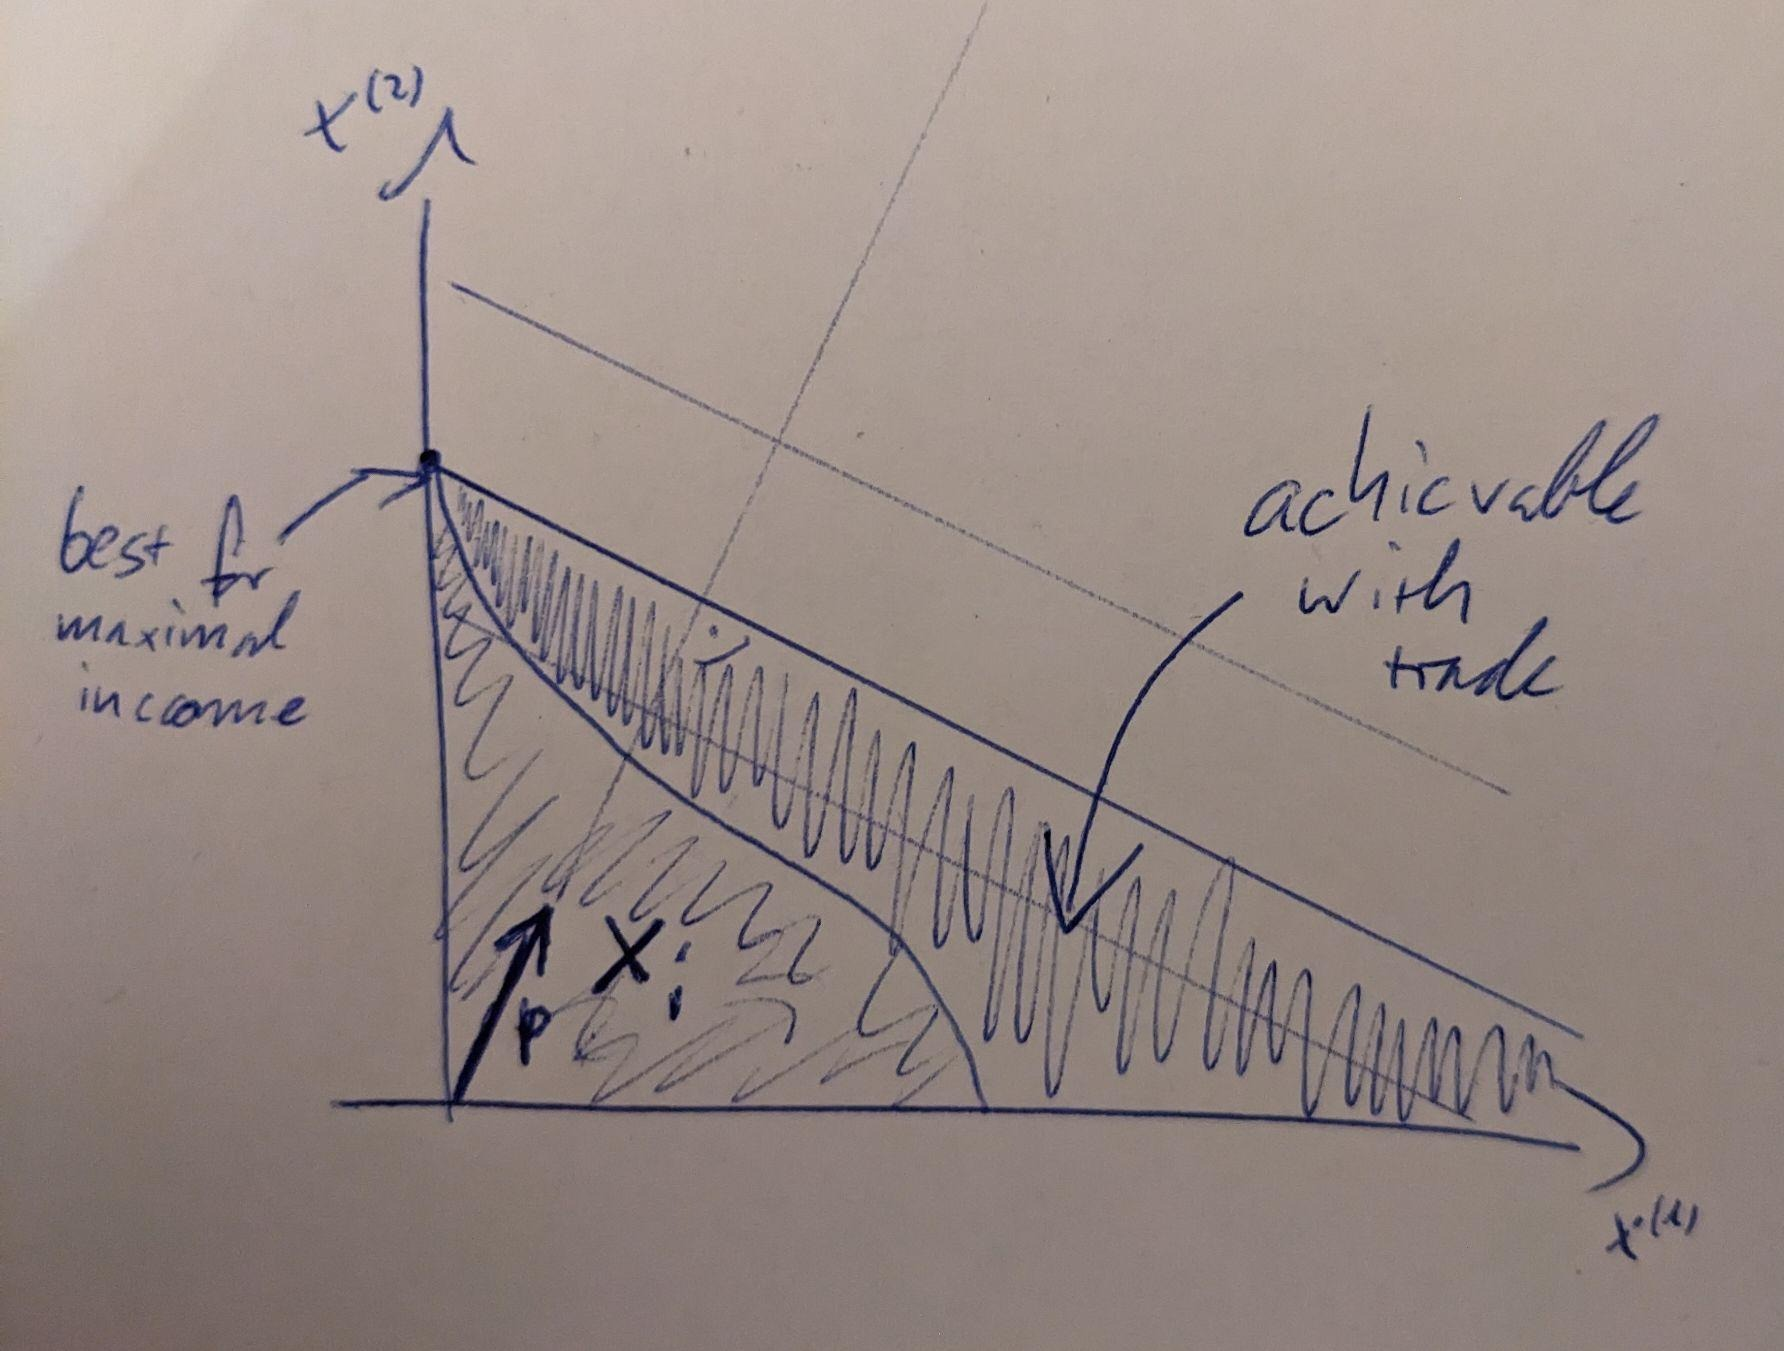
\includegraphics[width=0.7\textwidth]{images/consumption_increase_by_trade.jpeg}
	\caption{
		Product vectors on the \(d-1\) dimensional hyperplanes orthogonal to \(p\)
		cost the same amount and can therefore be exchanged (here \(d=2\), so the
		hyperplanes are lines). Trading at prices \(p\) enlarges the set of
		product vectors available for consumption for person \(i\).
	}
	\label{fig: consumption increase by trade}
\end{figure}
For a fixed price vector \(p\), let us consider the production and consumption
decision of person \(i\). As their expenses have to be smaller than their
income, it makes sense to maximize income for a given amount of labour \(L_i\).
Recall that our production options are \(X_i=X_i(L_i)\). So the maximal income
given labour \(L_i\) is
\[
	\tag{income}\label{eq: income}
	\mu(p, X_i) := \sup\{\langle p, x\rangle : x\in X_i\}.
\]
The function \(\mu(\cdot, X_i)\) in \(p\), is called the ``support function'' of
\(X_i\). It has some useful properties we will be grateful for later on. The
individual decision problem of person \(i\) therefore becomes
\begin{equation}
	\tag{IDP}
	\label{eq: individual decision problem}
	\max_{L_i, y} u(1-L_i, y) \quad\text{subject to}\quad \langle y, p\rangle \le \mu(p, X_i(L_i))
\end{equation}
In Figure~\ref{fig: consumption increase by trade} we can see, how this
constraint is always weaker than \(y\in X_i(L_i)\), which is the constraint of
self-sufficiency. I.e. we get the following lemma.

\begin{lemma}[Trade is never harmful]
\[
	\underbrace{X_i(L_i)}_{\text{own production}}
	\subseteq \quad
	\underbrace{
		\{y\in\real_{\ge 0}^\dims: \langle y, p\rangle \le \mu(p, X_i)\}
	}_{\text{consumption options with trade}}
\]
\end{lemma}
\begin{proof}
	Choose an arbitrary \(y\in X_i\), then by definition of \(\mu\)
	\[
		\langle p, y\rangle \overset{y\in X_i}\le \sup\{\langle p, x\rangle : x\in
		X_i\} \overset{\text{def.}}= \mu(p, X_i),
	\]
	\(y\) is also in the set on the right.
\end{proof}

\subsubsection{Income in Special Cases}

\begin{lemma}[Income in the Pure Variable Cost Case]
	In the pure variable cost case \(L_i(x) = \langle l_i, x\rangle\), income
	can be written as
	\[
		\mu(p, X_i(L_i))
		= \overbrace{L_i}^{\text{work time}} \max_{j=1,\dots,\dims}
		\underbrace{\frac{p_j}{l_i^{(j)}}}_{=: w_i^{(j)}}
		= L_i \overbrace{\|w_i\|_\infty}^{\text{wage}},
	\]
	where \(w_i^{(j)}\) are potential wages for producing good \(j\).
\end{lemma}
\begin{proof}
	Let \(H:= \diag(l_i)\), then as \(X_i\) is compact we know the supremum is
	a maximum and
	\begin{align*}
		\mu(p, X_i)
		&= \max_{x\ge 0} \langle p, x\rangle
		\text{ s.t. } \langle x, l_i\rangle \le L_i\\
		&\overset{y=Hx}= \max_{y\ge 0} \langle p, H^{-1}y\rangle
		\text{ s.t. } \underbrace{\langle H^{-1}y, l_i\rangle}_{
			= \langle y, 1 \rangle = \|y\|_1
		} \le L_i\\
		&= L_i \underbrace{
			\max_{y\ge 0} \langle H^{-1}p, y\rangle \text{ s.t. } \|y\|_1 \le 1
		}_{
			= \|H^{-1} p\|_{\text{Op-Norm(1)}} = \|H^{-1} p \|_\infty
		}\\
		&= L_i \max_{j=1,\dots,\dims} \frac{p_j}{l_i^{(j)}},
	\end{align*}
	where we have used, that all entries of \(y\) are non-negative when
	converting to the \(1\)-norm, \(\|x\|_1 = \sum_{i=1}^\dims |x_i|\), the
	fact that the operator norm of the \(1\)-norm is the sup norm
	\(\|x\|_\infty = \sup_{i=1,\dots,\dims} |x_i|\)\fxnote{source or appendix},
	and finally positivity of entries of \(p\) and \(l_i\) again.
\end{proof}

While the pure variable cost case already lends itself to specialization, unless
multiple wage options \(w_i^{(j)}\) are identical, adding fixed costs truly
encourages specialization. For fixed costs \(f_i\) the production capability
of person \(i\) can be written as 
\[
	X_i = \{
		x\in \real_{\ge 0}^\dims
		: \langle l_i, x\rangle
		+ \underbrace{
			\sum_{j=1}^\dims f_i^{(j)}\ind_{x^{(j)}>0}
		}_{=: \langle f_i, \ind_{>0}\rangle} \le L_i
	\}.
\]

\begin{lemma}[Income in Variable \& Fixed Cost Case]
	We assume the person is able to produce any product. So none of the fixed
	costs \(f_i^{(j)}\) take longer than the total labour time \(L_i\) (i.e.
	\(L_i - f_i^{(j)} > 0\)). In this mixed case, income of person \(i\) can be
	written as		
	\[
		\mu(p, X_i)
		= L_i \max_{j=1,\dots,d}\underbrace{\frac{p_j}{\bar{l}_i^{(j)}}}_{=:w_i^{(j)}}
		= L_i \|w_i\|_\infty,
	\]
	where the average labour cost \(\bar{l}_i^{(j)}\) of person \(i\) of
	specialization \(j\) is given by
	\[
		\bar{l}_i^{(j)}
		:= l_i^{(j)}\frac{L_i}{L_i-f_i^{(j)}}
		= l_i^{(j)}\frac{1}{1-f_i^{(j)}/L_i}
	\]
\end{lemma}
\begin{proof}
	For a subset \(J\subseteq\{1,\dots,\dims\}\) define the subspace
	\[
		\real_{>0}^J:= \{
			x\in \real^\dims:
			x^{(j)} > 0\ \forall j\in J;\;\; x_j =0\ \forall j\notin J
		\}.
	\]
	Then we can partition our maximization problem by these \(J\) like this:
	\begin{align*}
		\mu(p, X_i)
		&= \max_{x\ge 0}\langle p, x\rangle \text{ s.t. }
		\langle x, l_i\rangle  + \langle f_i, \ind_{>0}\rangle \le L_i\\
		&= \max_{J \subseteq \{1,\dots,\dims\}}
		\max_{x\in \real_{>0}^J}
		\langle p, x\rangle \text{ s.t. } \langle x, l_i\rangle \le L_i - \sum_{j\in J}f_i^{(j)}
	\end{align*}	
	We can relax the inner maximization problem to obtain the pure variable
	optimization problem embedded in \(\real^I\)
	\begin{align*}
		&\max_{x\in \real_{>0}^J}
		\langle p, x\rangle \text{ s.t. }
		\langle x, l_i\rangle \le L_i - \sum_{j\in J}f_i^{(j)}\\
		&\le 
		\max_{x\in \real_{{\color{red} \ge} 0}^J}
		\langle p, x\rangle \text{ s.t. }
		\langle x, l_i\rangle \le L_i - \sum_{j\in J}f_i^{(j)}\\
		&= \Bigl(L_i - \sum_{j\in J}f_i^{(j)}\Bigr)
		\max_{j\in J} \frac{p_j}{l_i^{(j)}}
	\end{align*}
	So in total, we have
	\begin{align*}
		\mu(p, X_i)
		&\le \max_{\emptyset \neq J\subseteq \{1,\dots,\dims\}}
		\Bigl(L_i - \sum_{j\in J}f_i^{(j)}\Bigr)
		\max_{j\in J} \frac{p_j}{l_i^{(j)}}\\
		&= \max_{j=1,\dots,\dims}
		(L_i - f_i^{(j)}) \frac{p_j}{l_i^{(j)}}.
	\end{align*}
	To see that this upper bound is actually tight, consider producing
	exclusively \(j\). Then we have
	\[
		l_i^{(j)} x^{(j)} + f_i^{(j)} = L_i \iff x^{(j)} = \frac{L_i-f_i^{(j)}}{l_i^{(j)}}.
	\]
	Optimizing over different specializations yields
	\[
		\mu(p, X_i) \ge \max_{j=1,\dots,\dims} p_j x^{(j)}
		= \max_{j=1,\dots,\dims}
		p_j \frac{L_i - f_i^{(j)}}{l_i^{(j)}}
		= L_i\max_{j=1,\dots,\dims}
		\frac{p_j}{l_i^{(j)}\frac{L_i}{L_i - f_i^{(j)}}}.
	\]
	Lastly the average labour cost of specialization \(j\) is given by
	\begin{align*}
		\bar{l}_i^{(j)}
		&= \frac{L_i}{x^{(j)}}
		= \frac{l_i^{(j)} x^{(j)} + f_i^{(j)}}{x^{(j)}}
		= l_i^{(j)} + \frac{f_i^{j}}{\left(\frac{L_i-f_i^{(j)}}{l_i^{(j)}}\right)}
		= l_i^{(j)} \Bigl[1 + \frac{f_i^{j}}{L_i-f_i^{(j)}}\Bigr]\\
		&=l_i^{(j)}\frac{L_i}{L_i - f_i^{(j)}}.
		\qedhere
	\end{align*}
\end{proof}

\subsubsection{The Individual Decision Problem in the Mixed Case}

By talking about average costs \(\bar{l}_i^{(j)}\) in place of variable costs
\(l_i^{(j)}\), we therefore salvaged the results from the pure variable
cost case. But no matter how the wage \(\|w_i\|_\infty\) comes to be, the
individual decision problem \eqref{eq: individual decision problem} becomes
\[
	\max_{L_i, y} u(1-L_i, y) \text{ s.t. } \langle p, y\rangle \le L_i \|w_i\|_\infty
\]
or in other words
\[
	\max_{y} u\left(1- \frac{\langle p, y\rangle}{\|w_i\|_\infty}, y\right).
\]
The first order condition is therefore
\[
	\frac{du}{dy} 
	= u_f\Bigl[
		\underbrace{\frac{u_y}{u_f}}_{\text{wtw}}
		- \overbrace{\frac{p}{\|w_i\|_\infty}}^{\text{effort required}}
	\Bigr]
	= \frac{u_f}{\|w_i\|_\infty}\Bigl[
		\underbrace{\frac{u_y}{u_f}\|w_i\|_\infty}_{\text{wtp}}
		- p
	\Bigr]
\]
Where the ``willingness to pay'' (wtp) is simply the willingness to work
(wtw) scaled by person \(i\)'s wages.

Careful readers might have noticed, that
this calculation is not quite accurate in the mixed case. Because the average costs
depend on \(L_i\), which in turn makes \(\|w_i\|_\infty\) dependent on \(L_i\).
So by the product rule, the effort required would be
\[
		\frac{dL_i}{dy}
		= \frac{d}{dy} \frac{\langle p, y\rangle}{\|w_i\|_\infty}
		= \frac{p}{\|w_i\|_\infty}
		- \frac{\langle p, y\rangle}{\|w_i\|_\infty^2}
		\frac{d\|w_i\|_\infty}{dL_i}\frac{dL_i}{dy}
\]
Joining the \(\frac{dL_i}{dy}\) on both sides results in
\[
	\frac{dL_i}{dy}
	= \frac{\frac{p}{\|w_i\|_\infty}}{
		1 + \frac{\langle p, y\rangle}{\|w_i\|_\infty^2}
		\frac{d\|w_i\|_\infty}{dL_i}
	}
	= \frac{p}{
		\|w_i\|_\infty + \frac{\langle p, y\rangle}{\|w_i\|_\infty}
		\frac{d\|w_i\|_\infty}{dL_i}
	}.
\]
Where \(\|w_i\|_\infty=\max_{j} w_i^{(j)}\) is piecewise differentiable with derivatives
\[
	\frac{dw_i^{(j)}}{dL_i}
	= \frac{d}{dL_i} \frac{p_j}{\bar{l}_i^{(j)}}
	= \frac{p_j}{l_i^{(j)}} \frac{d}{dL_i} \frac{L_i-f_i^{(j)}}{L_i}
	= \frac{p_j}{l_i^{(j)}} \frac{f_i^{(j)}}{L_i^2} > 0.
\]
In other words: Wages increase with total labour time \(L_i\), as
average cost decrease with \(L_i\). The size of this effect increases with the
size of the fixed costs. If the fixed costs are close to \(L_i\) small decreases
of \(L_i\) might make producing \(j\) completely unviable, but at the very least
cut heavily into the little time left for actually producing \(j\). In fact
average costs have singularities at \(f_i^{(j)}\)
\[
	\lim_{L_i\downarrow f_i^{(j)}} \bar{l}_i^{(j)}
	= \lim_{L_i\downarrow f_i^{(j)}}l_i^{(j)}\frac{1}{1-f_i^{(j)}/L_i}
	= \infty.
\]
Using \(\bar{l}_i^{(j)}=l_i^{(j)}\frac{L_i}{L_i-f_i^{(j)}}\) we can alternatively
write
\[
	\frac{dw_i^{(j)}}{dL_i}
	= \frac{p_j}{\bar{l}_i^{(j)}} \frac{f_i^{(j)}(L_i-f_i^{(j)})}{L_i}
	= w_i^{(j)} \frac{f_i^{(j)}(L_i-f_i^{(j)})}{L_i}.
\]
With \(j^* := \argmax_{j} w_i^{(j)}\) and \(L_i = \frac{\langle p,
y\rangle}{\|w_i\|_\infty}\), this finally results in the effort required
\[
	\frac{dL_i}{dy}
	= \frac{p}{
		\|w_i\|_\infty + \langle p, y\rangle f_i^{(j^*)}
		\bigl(1-\frac{f_i^{(j^*)}}{L_i}\bigr)
	}
	= \frac{p}{
		\|w_i\|_\infty + f_i^{(j^*)}
		\bigl(\langle p, y\rangle-f_i^{(j^*)}\|w_i\|_\infty\bigr)
	}.
\]
The willingness to pay is therefore given by
\[
	\text{wtp} = \frac{u_y}{u_f}\Bigl[
		\|w_i\|_\infty + f_i^{(j^*)}
		\bigl(\langle p, y\rangle-f_i^{(j^*)}\|w_i\|_\infty\bigr)
	\Bigr].
\]

\subsection{Prices in Societies of Clones}

\begin{example*}[Pure Variable Cost case with Identical Production Capabilities]

\end{example*}